\section{Introduction}

\begin{frame}
\frametitle{Introduction}
\framesubtitle{Driver Monitoring Systems}

Modern \textit{driver monitoring systems} (DMSs) in Level-2+ self-driving-enabled cars aim to enhance safety by estimating drivers' readiness levels for driving and enabling safe control handovers when necessary.

\begin{figure}[hb]
    \centering
    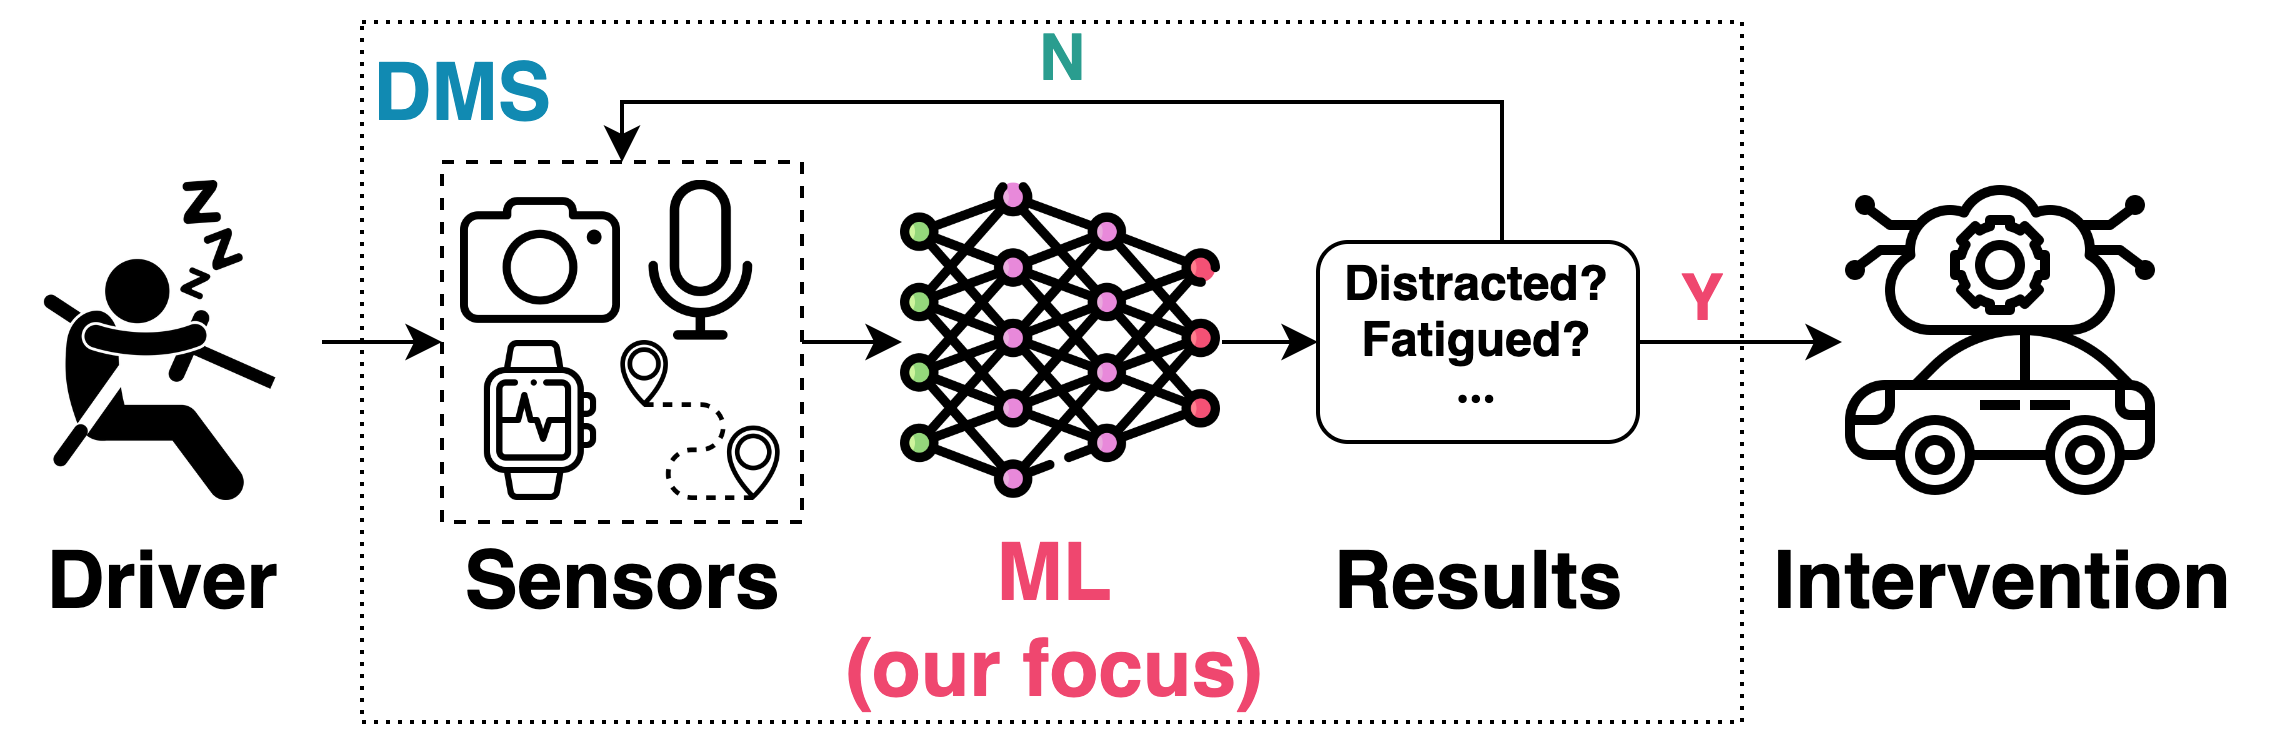
\includegraphics[width=0.9\linewidth]{images/dms.png}
    \caption{A simplified illustration of a DMS.}
    \label{fig:1}
\end{figure}
\end{frame}

\begin{frame}
\frametitle{Introduction}
\framesubtitle{Driver Monitoring Systems}

These systems usually rely various sensors, which may be deployed at different in-car locations, to comprehensively monitor drivers' states, e.g.,

\begin{itemize}
    \item \textbf{RGB}: optical details.
    \item \textbf{Depth}: 3D information.
    \item \textbf{Infrared}: thermal information.
    \item \textbf{ECG}: heart rates.
    \item \textbf{Audio}: speech and sound.
\end{itemize}

Hence, modern DMSs are \textit{multimodal} (and \textit{multiview}).
\end{frame}

\begin{frame}
\frametitle{Introduction}
\framesubtitle{Our Work}

Our work specifically focuses on \textit{driver action recognition}, which involves classifying drivers' actions into \textit{normal driving} and several \textit{non-driving-related activities} (NDRAs), e.g., texting and drinking.

\begin{figure}
    \centering
    \begin{subfigure}[b]{0.24\textwidth}
        \centering
        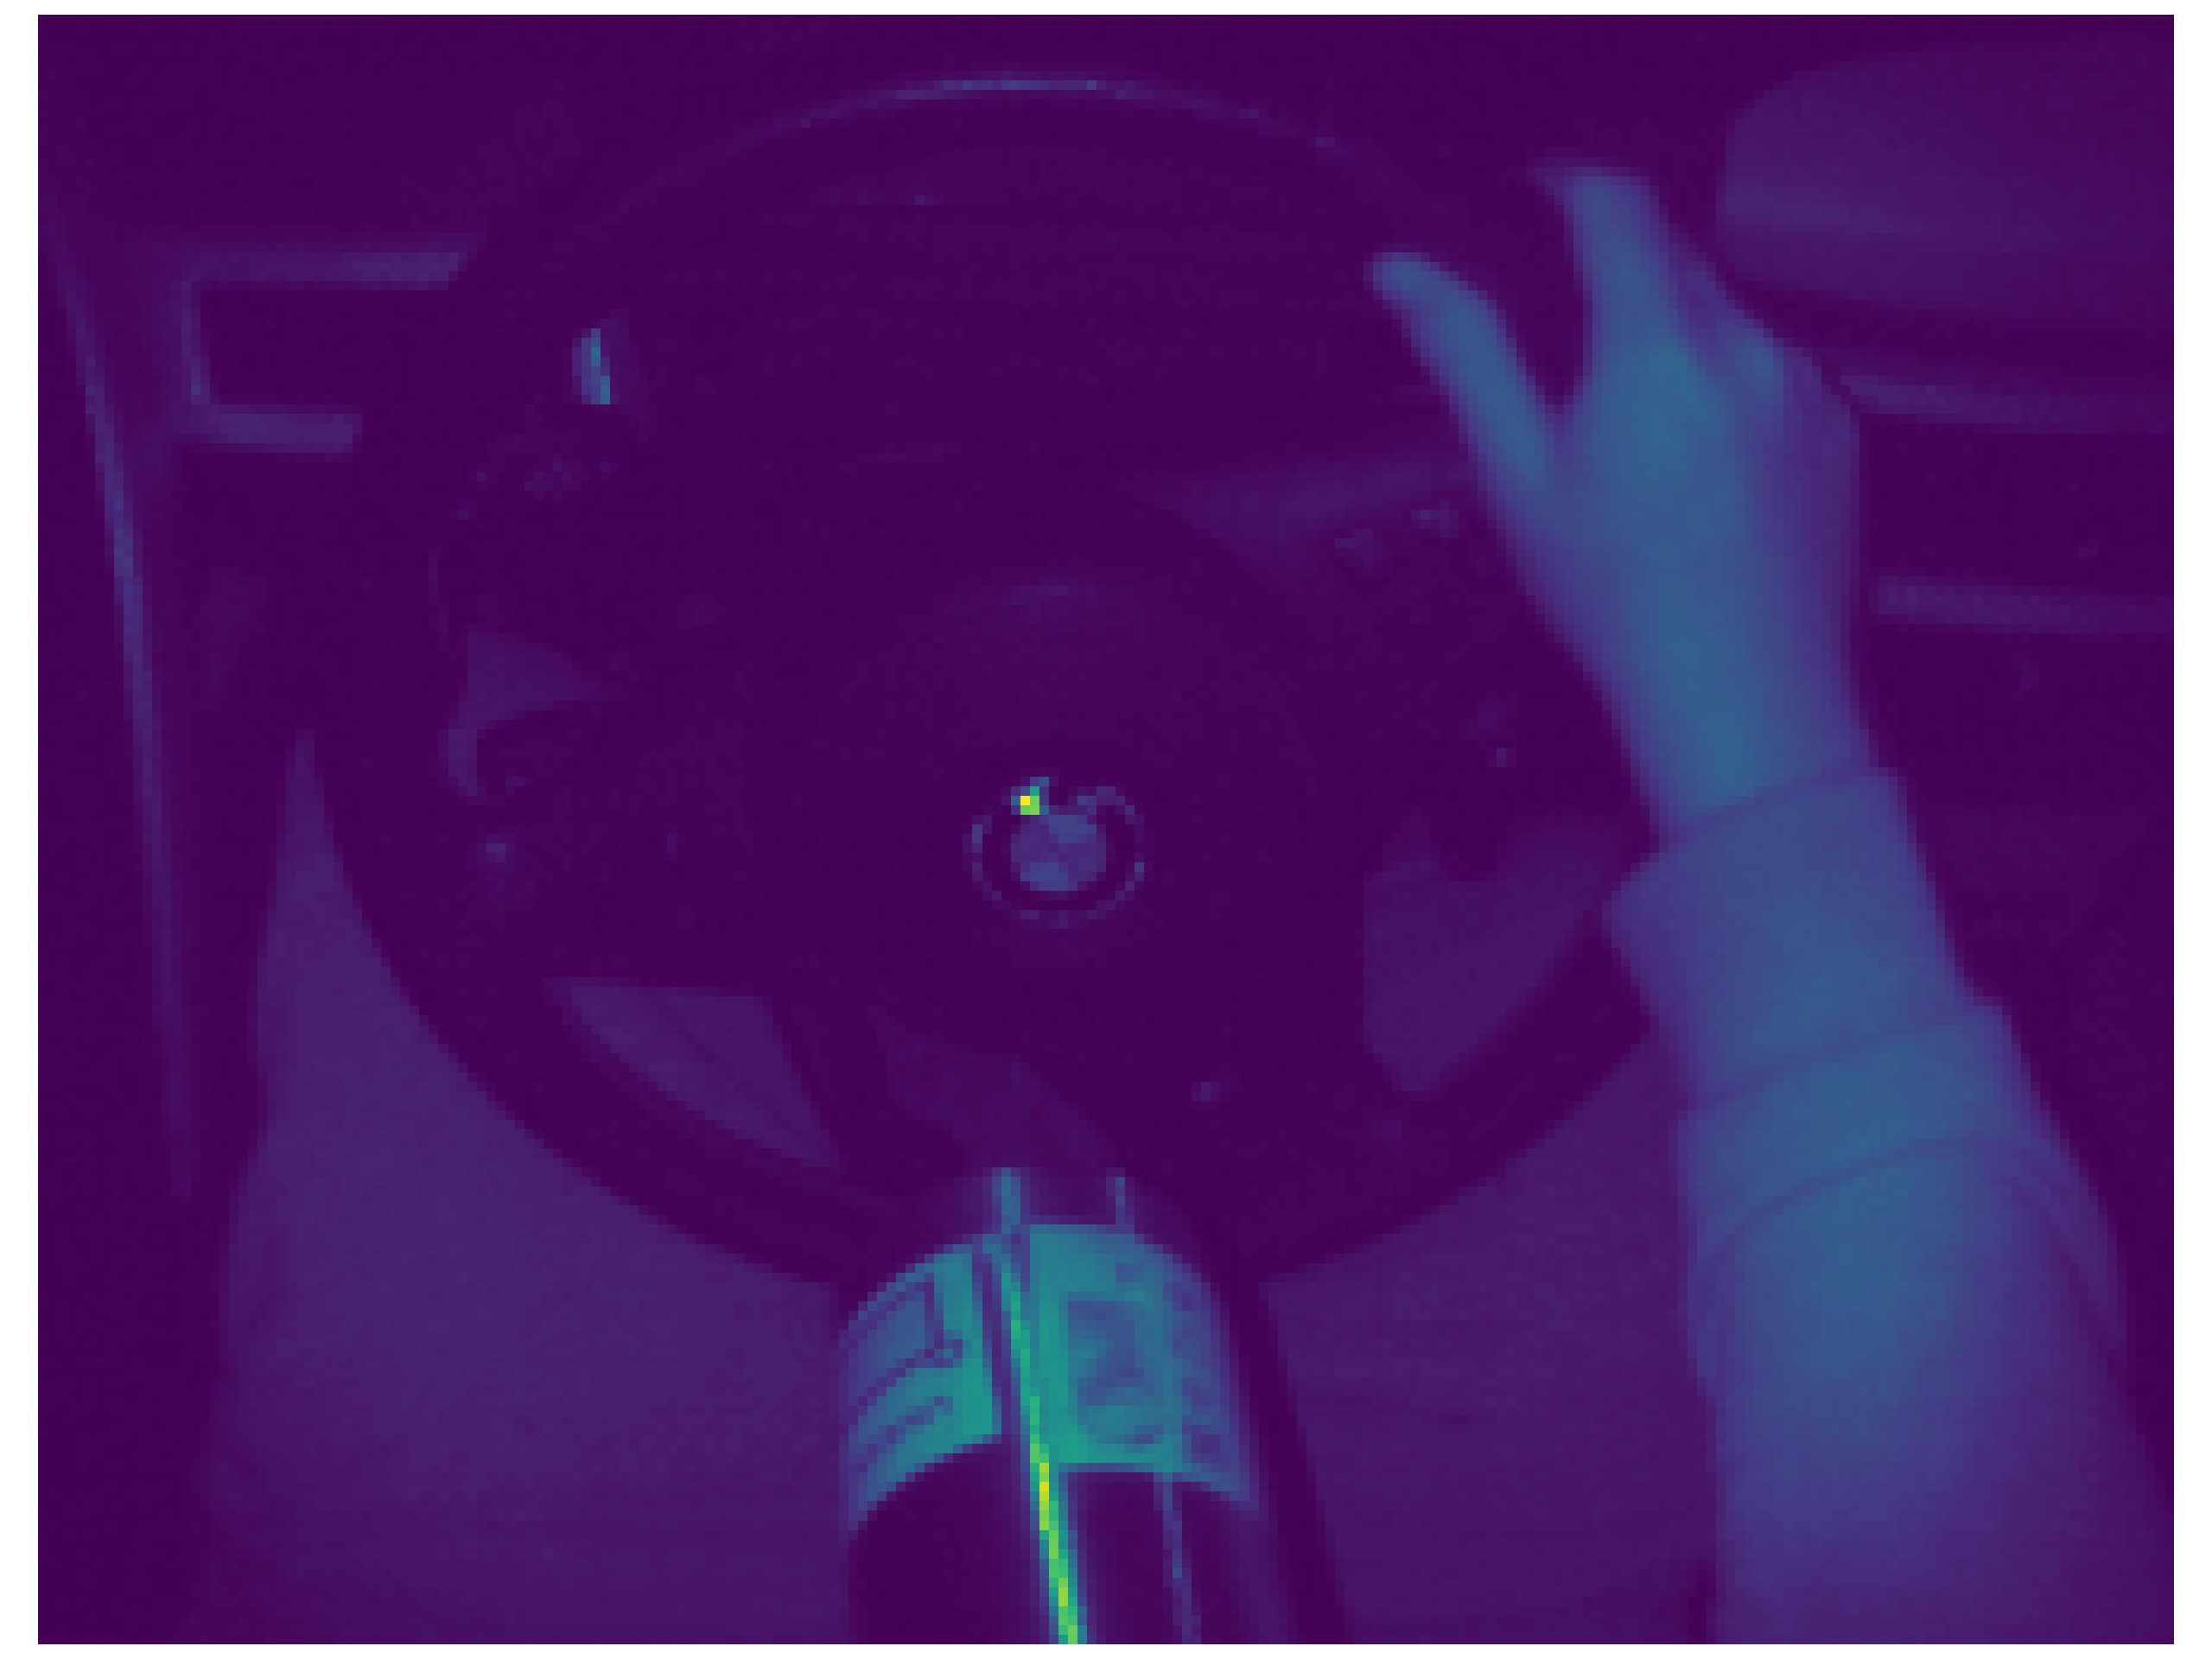
\includegraphics[width=\textwidth]{images/dad_top_ir.png}
        \caption{Top IR}
        \label{fig:2.a}
    \end{subfigure}
    \hfill
    \begin{subfigure}[b]{0.24\textwidth}
        \centering
        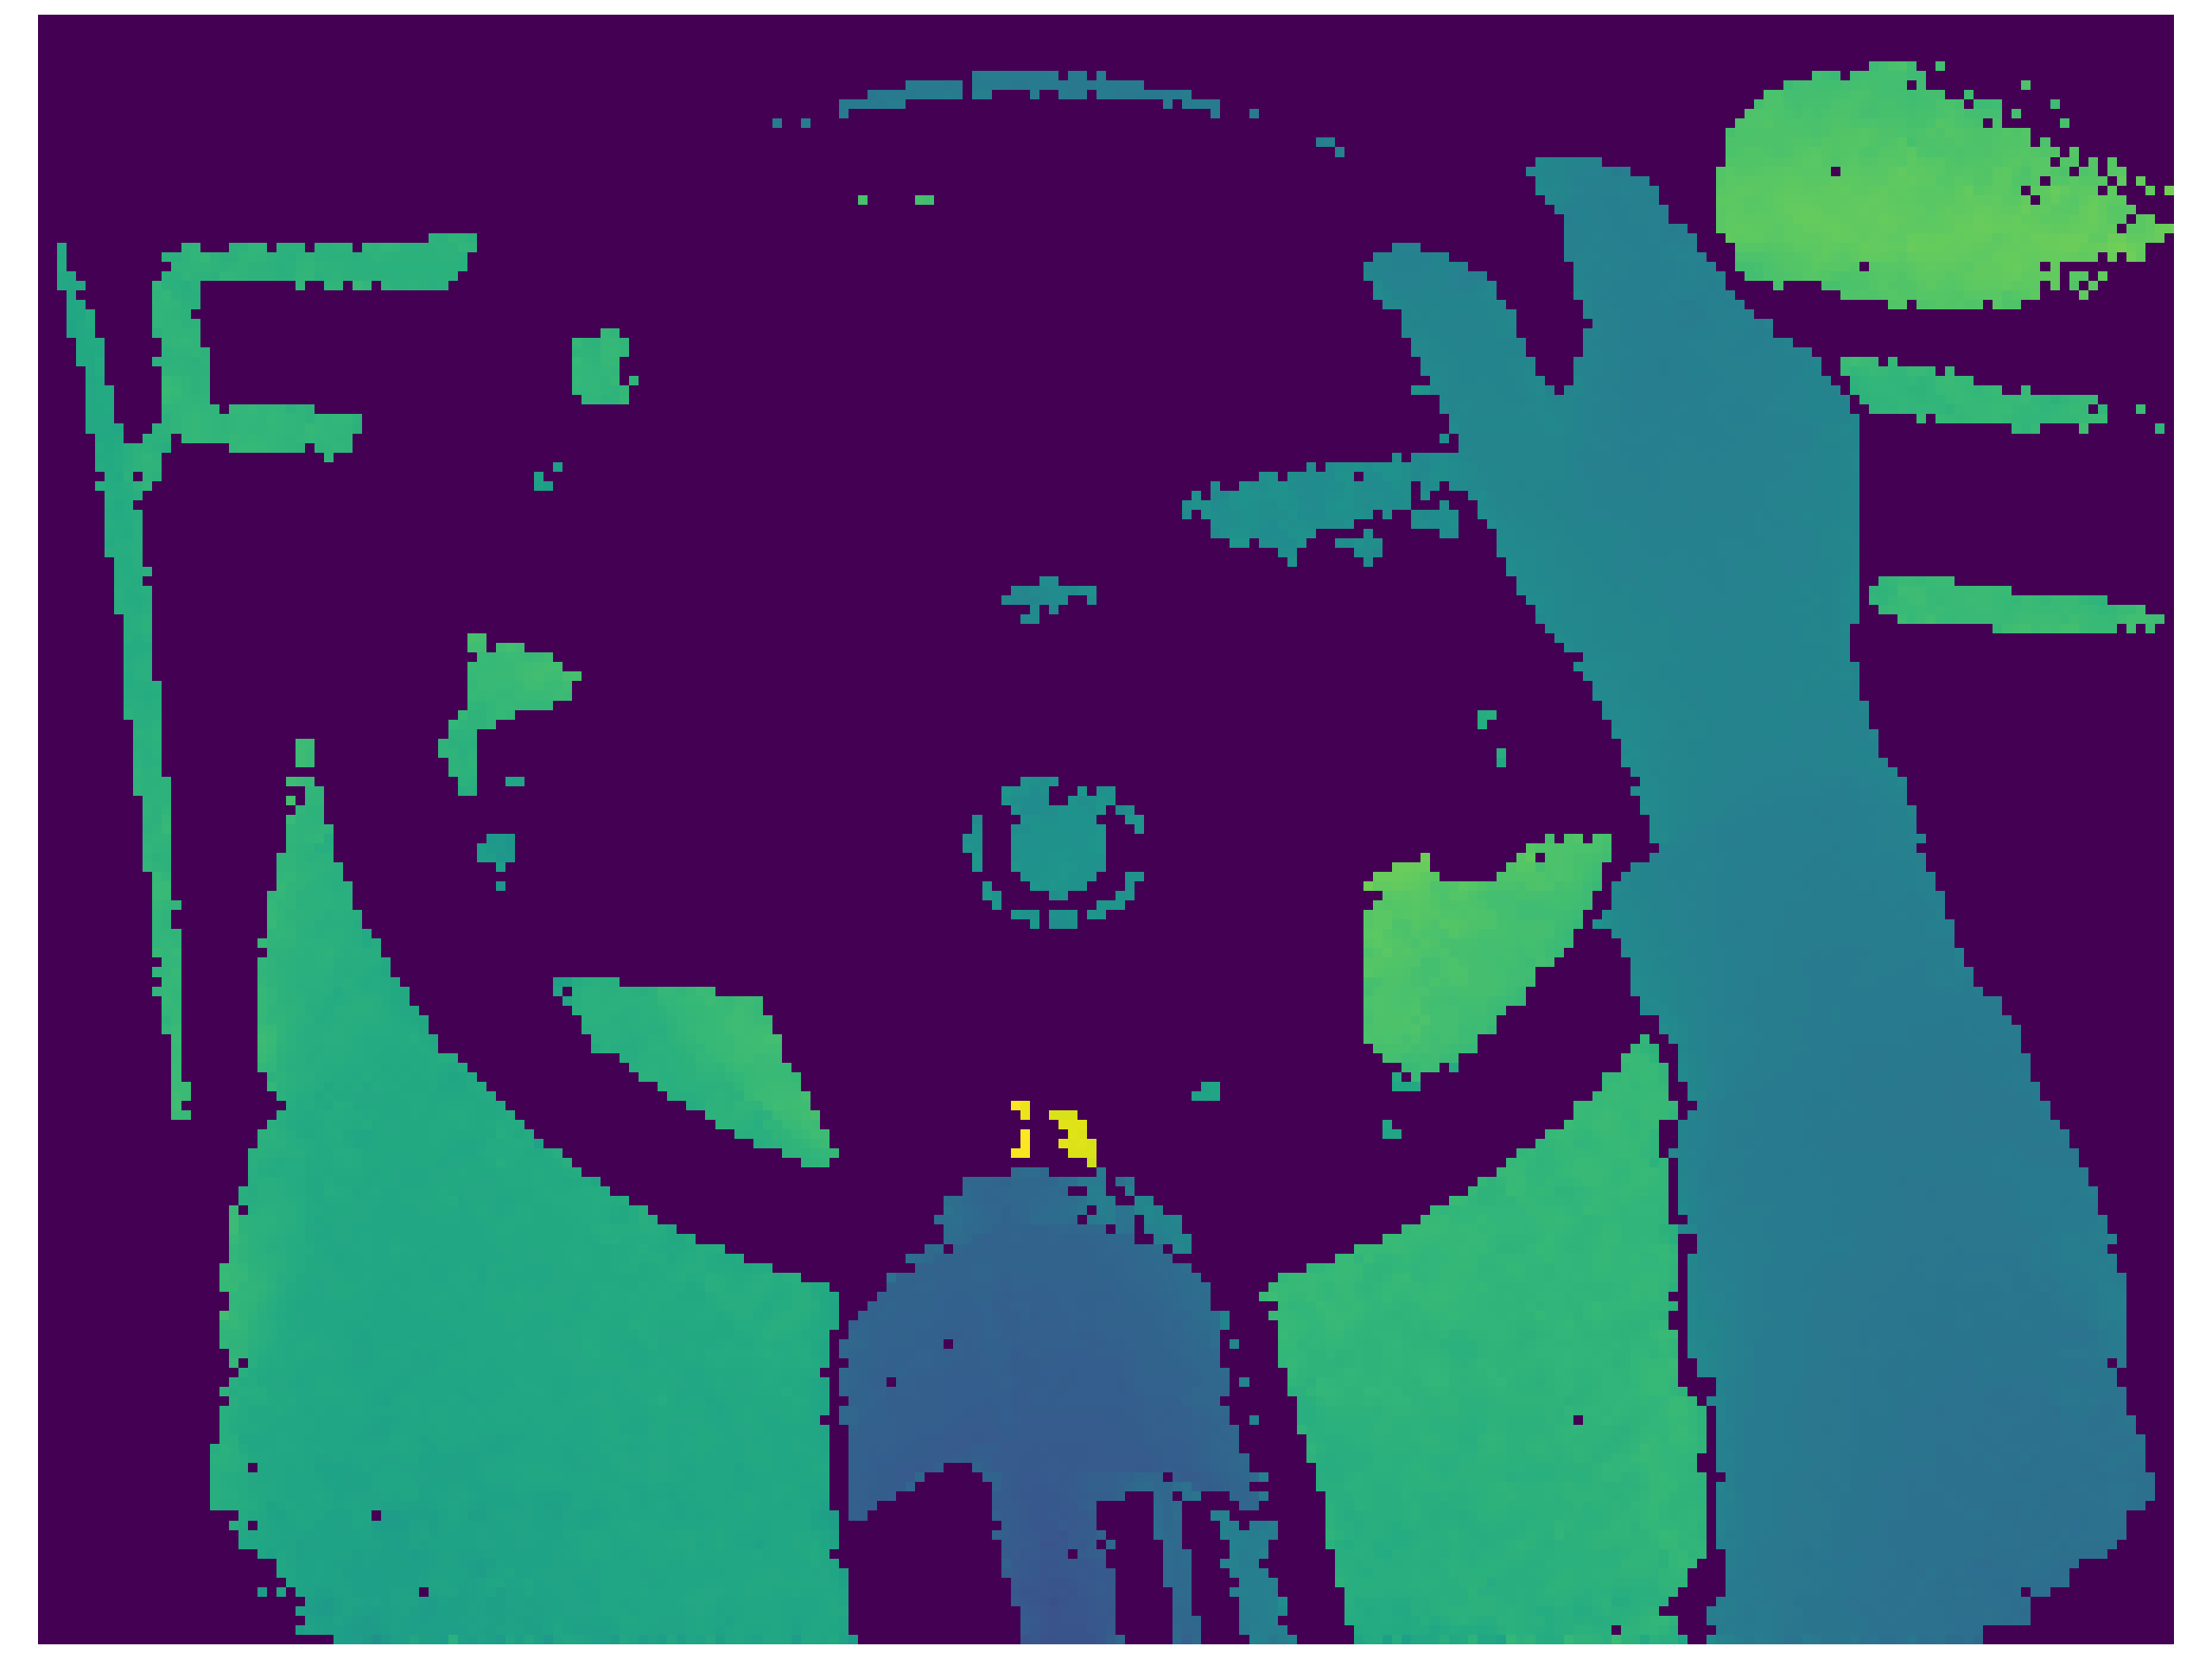
\includegraphics[width=\textwidth]{images/dad_top_depth.png}
        \caption{Top Depth}
        \label{fig:2.b}
    \end{subfigure}
    \hfill
    \begin{subfigure}[b]{0.24\textwidth}
        \centering
        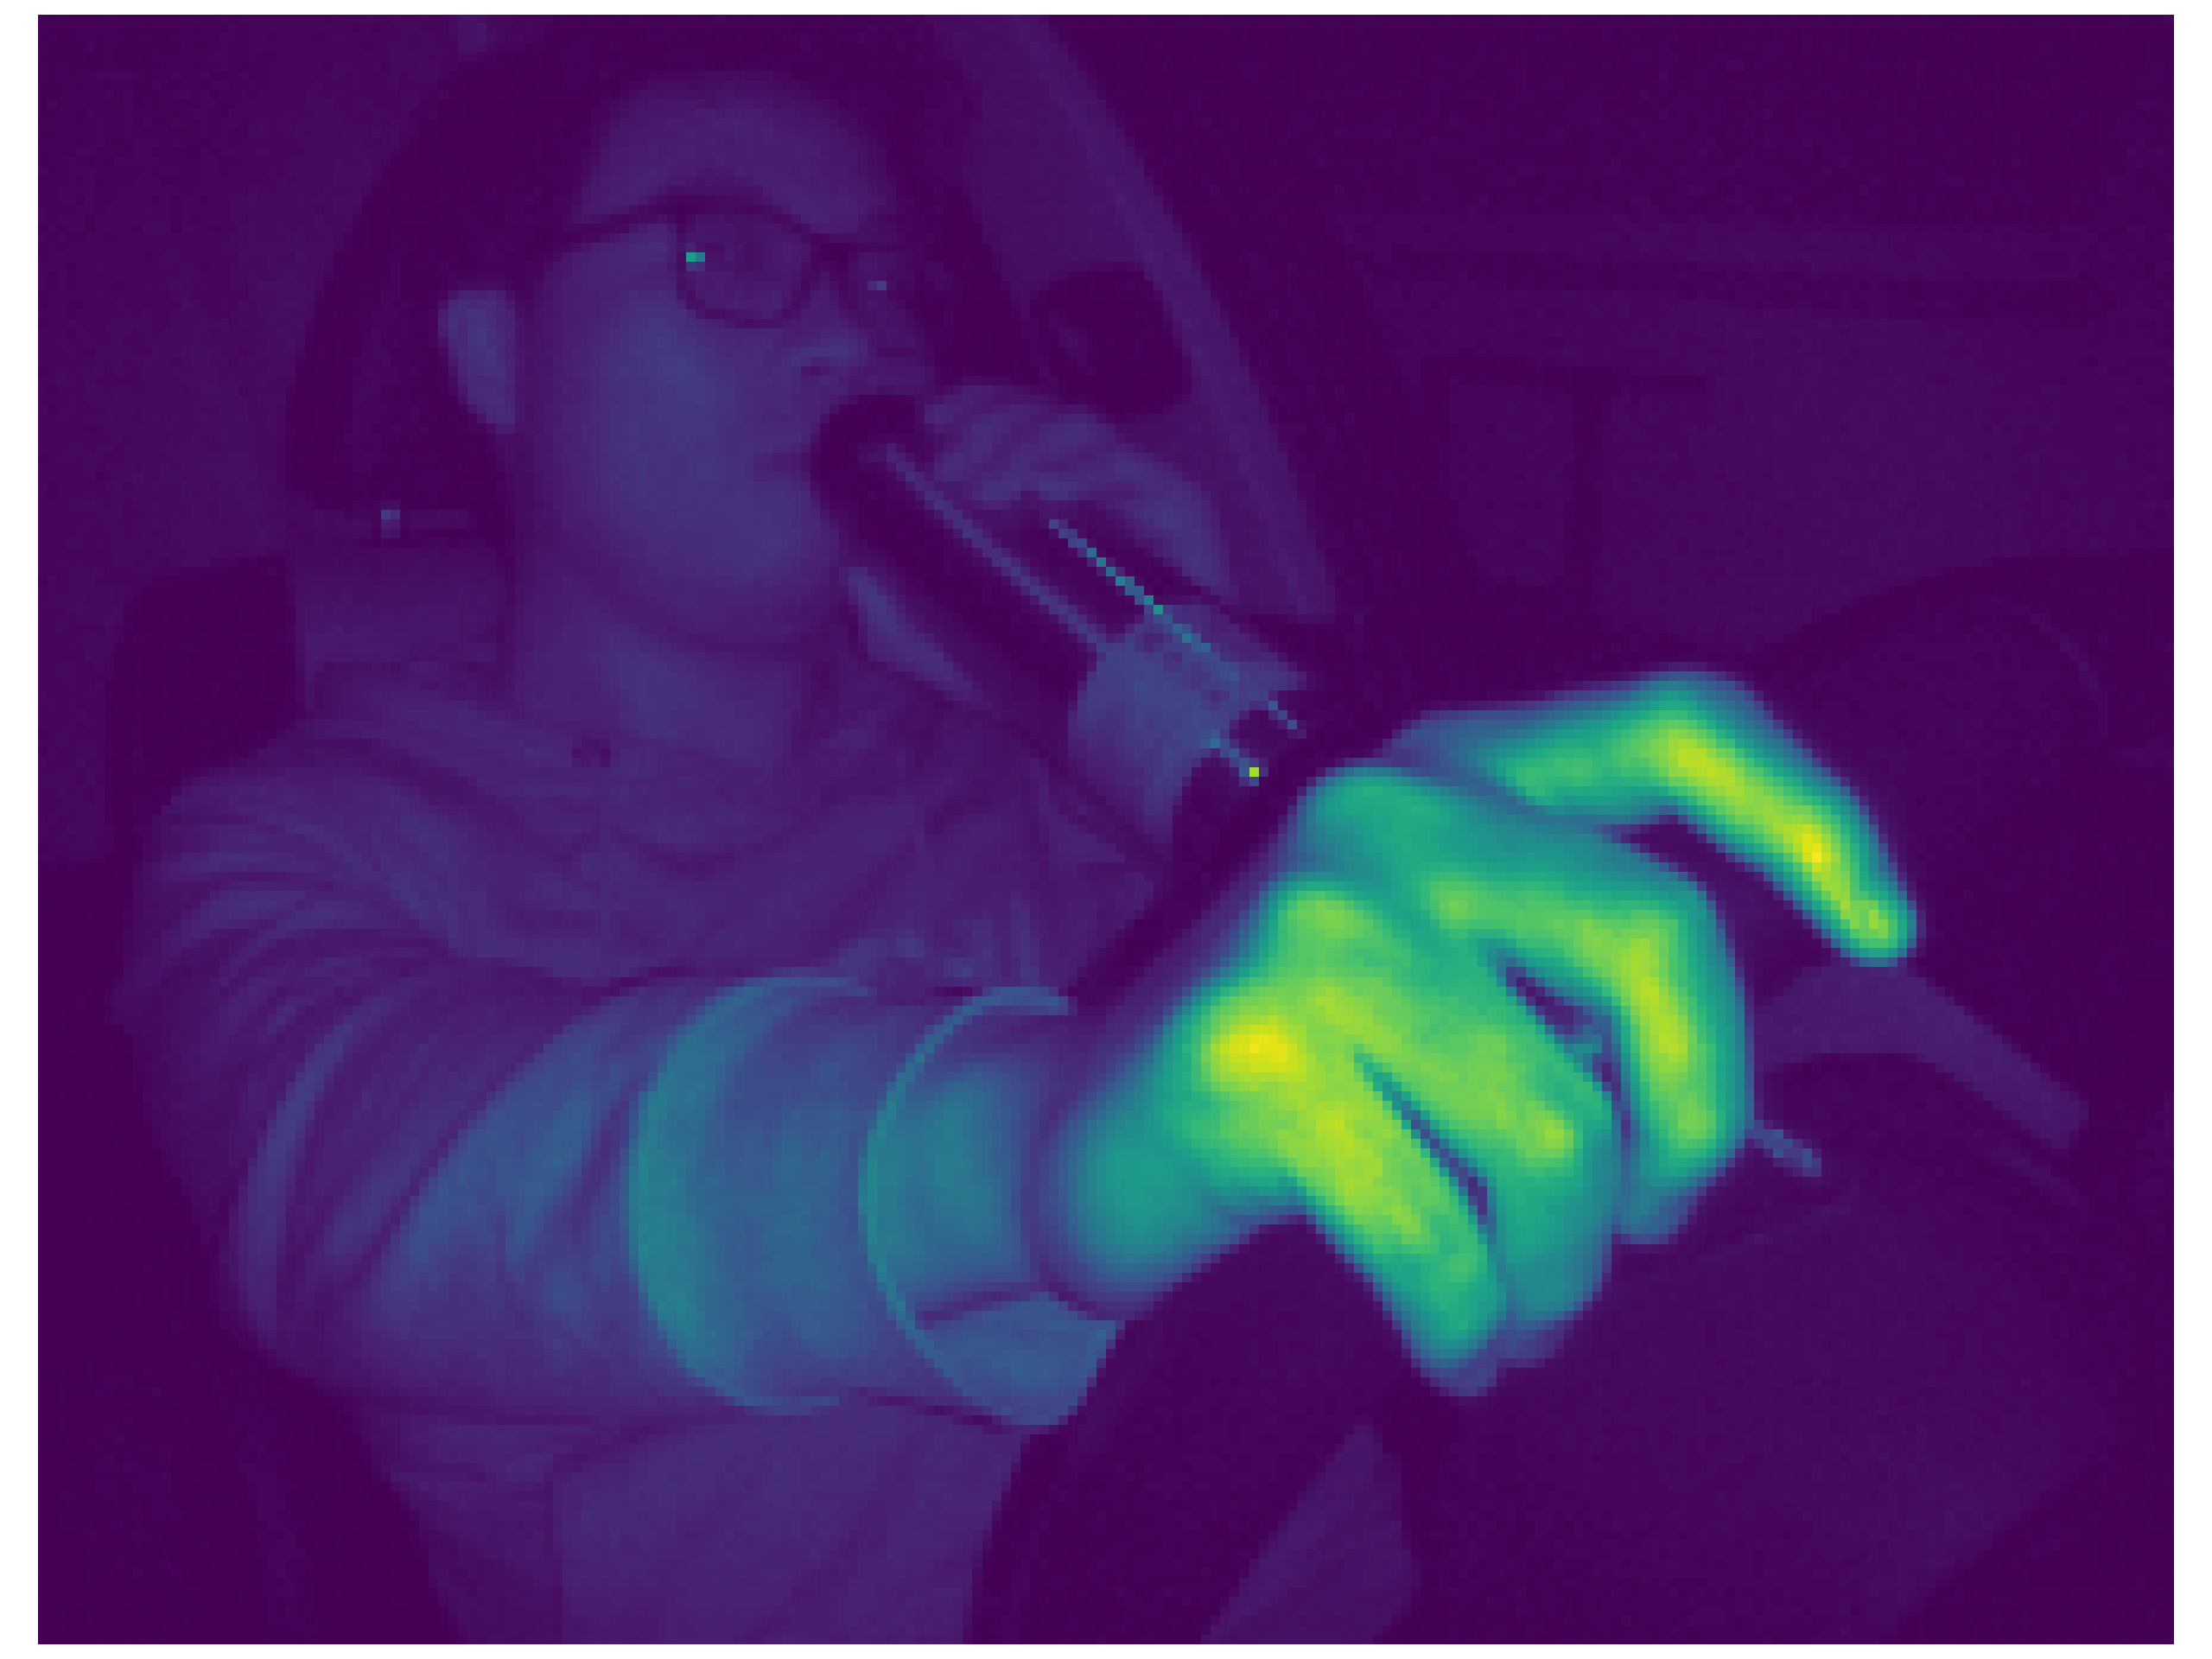
\includegraphics[width=\textwidth]{images/dad_front_ir.png}
        \caption{Front IR}
        \label{fig:2.c}
    \end{subfigure}
    \hfill
    \begin{subfigure}[b]{0.24\textwidth}
        \centering
        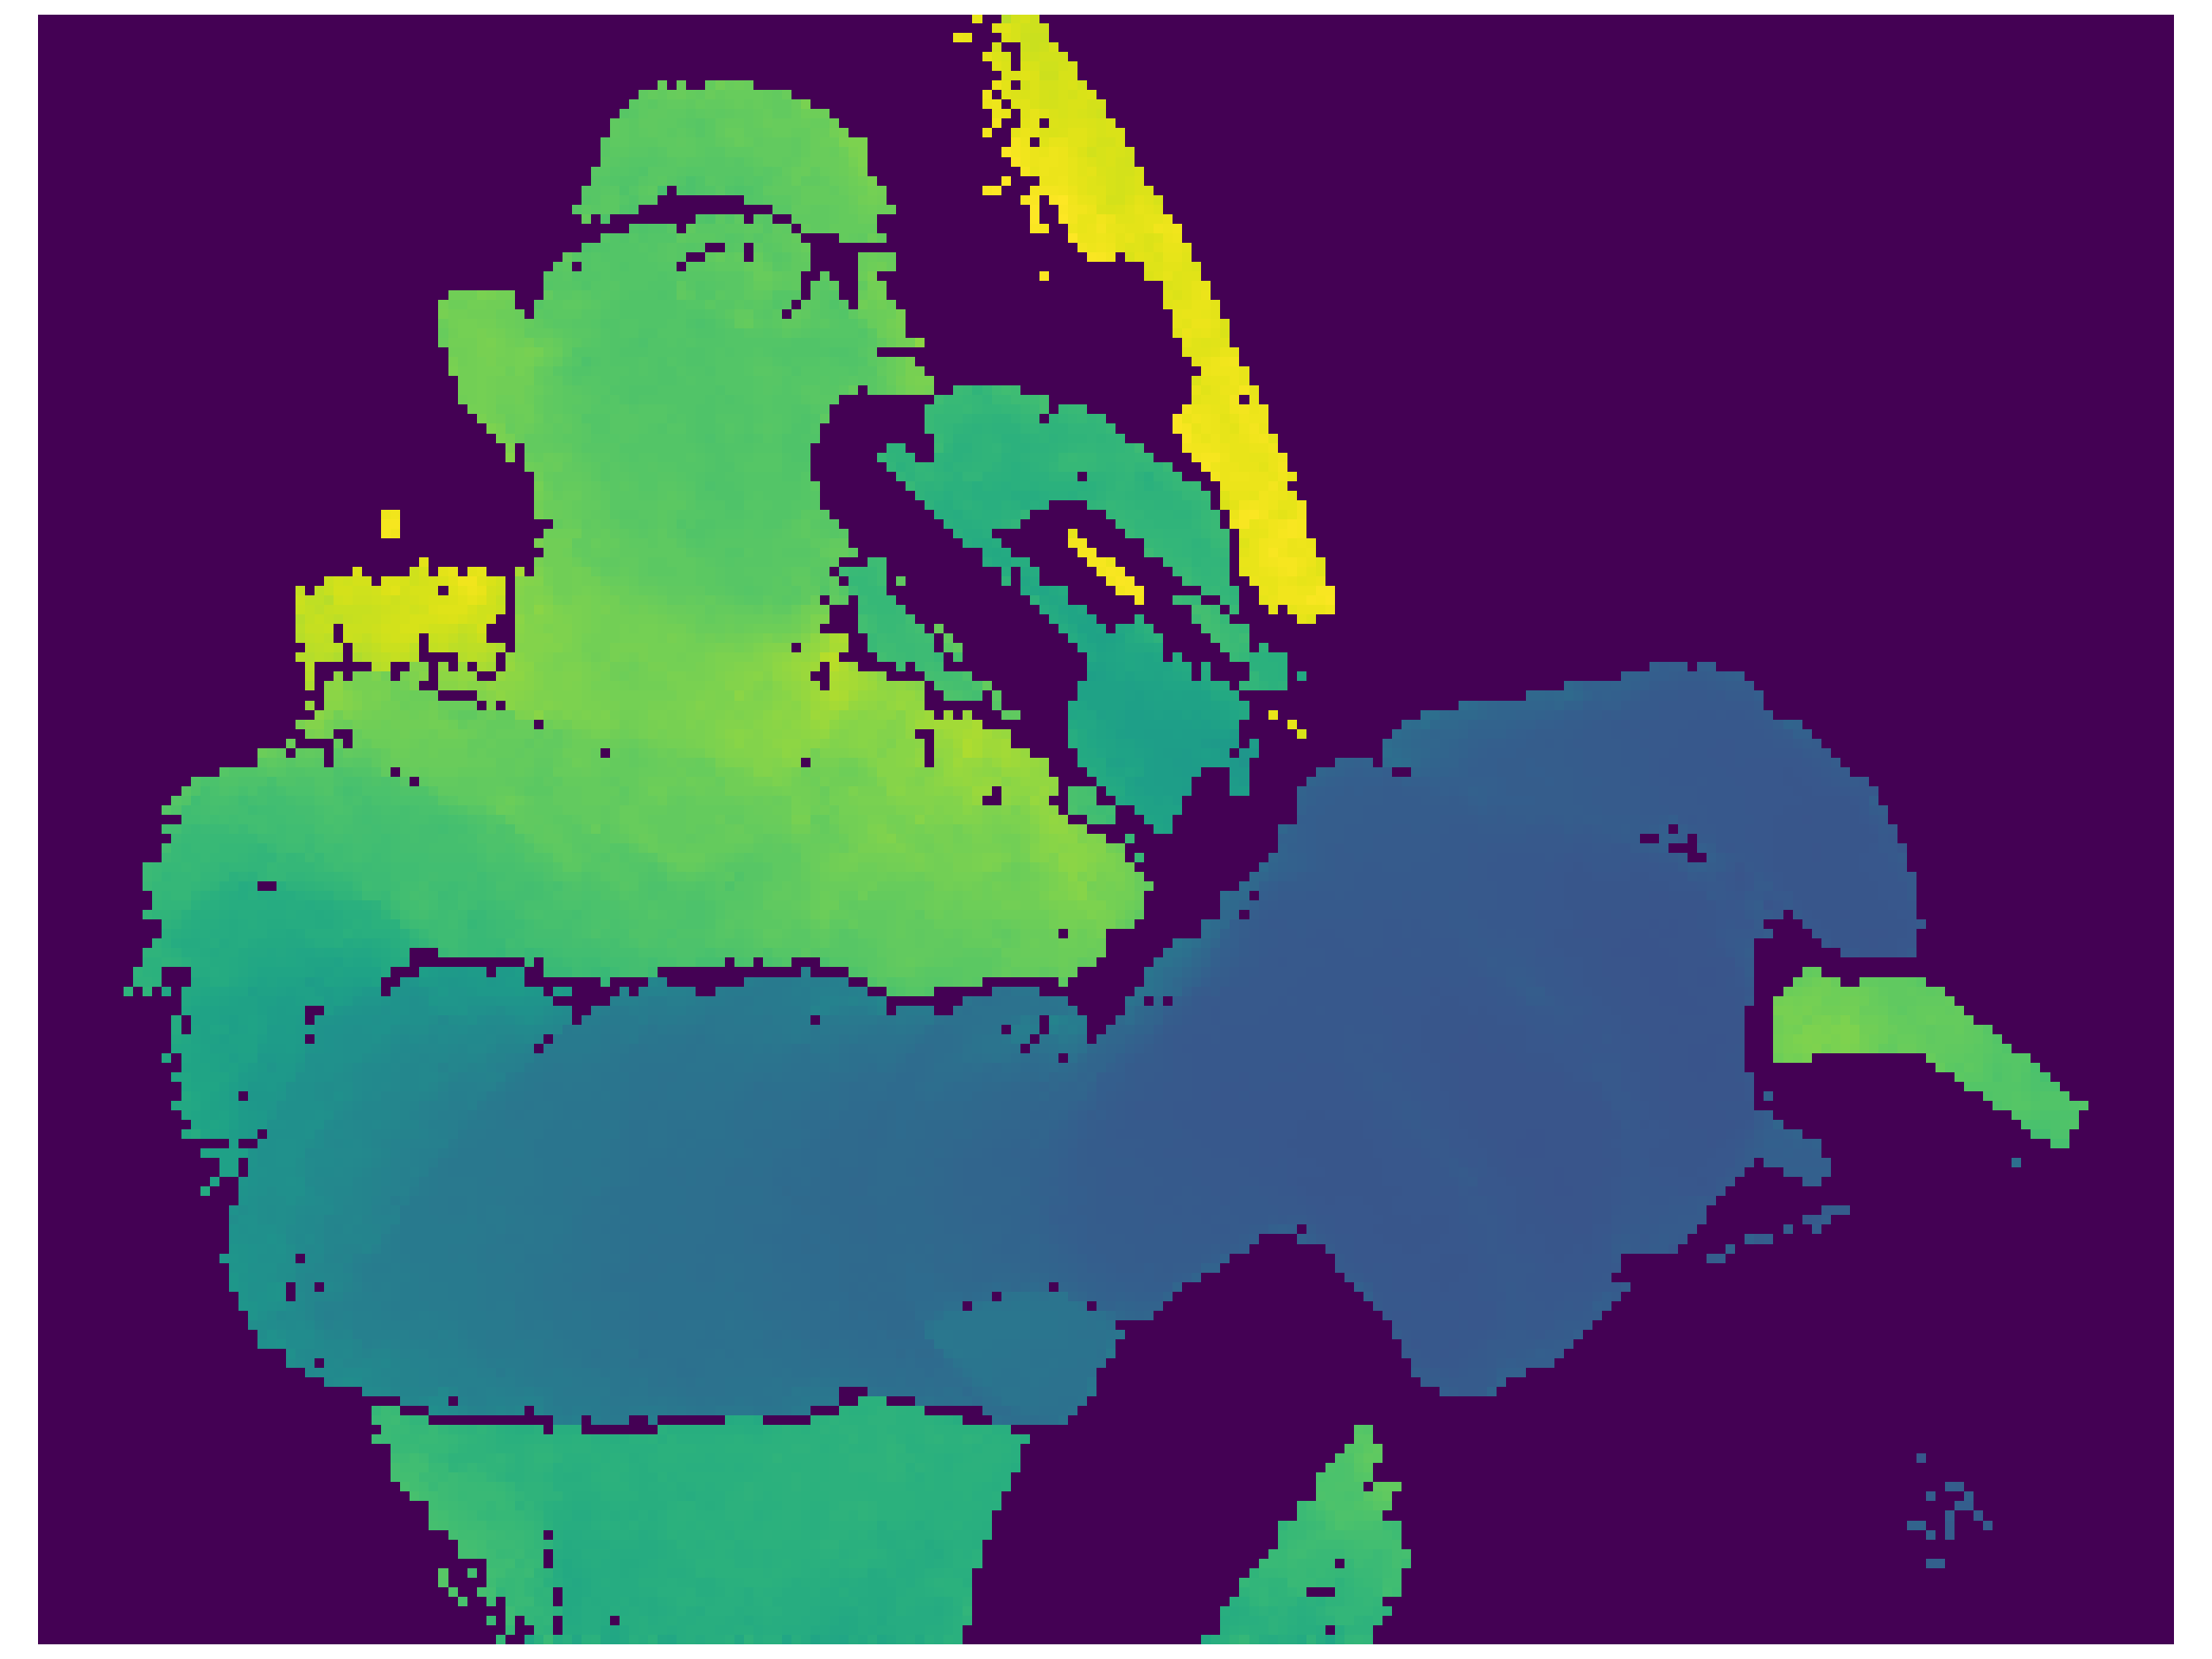
\includegraphics[width=\textwidth]{images/dad_front_depth.png}
        \caption{Front Depth}
        \label{fig:2.d}
    \end{subfigure}
    \caption{Sample frames from the DAD dataset \cite{kopuklu2021driver}.}
    \label{fig:2}
\end{figure}

\end{frame}

\begin{frame}
\frametitle{Introduction}
\framesubtitle{Our Work}
    Our contributions in this paper are as follows:
    \begin{enumerate}
        \item We propose a novel robust \textit{multiview multimodal} DMS for driver action recognition that leverages feature-level fusion through masked \textit{multi-head self-attention} (\textbf{MHSA}).
        \item We manually annotated the anomalies in DAD dataset with 9 fine-grained classes of non-driving-related activities (NDRAs).
        \item We conduct extensive experiments on the DAD dataset to compare different fusion strategies, assess the significance of individual views/modalities, and evaluate the efficacy of patch masking in enhancing MHSA's robustness against view/modality collapses. Results show that our MHSA-based DMS achieves state-of-the-art performance with an AUC-ROC score of \underline{97.0\%}. 
    \end{enumerate}
\end{frame}